\section{Results}
\label{sec:results}

We present the empirical preconditions first (terrain, wind, lift), then the
model-dependent flight dynamics and synthesis.

\subsection{The abbey sits on a wind-aligned escarpment}

The abbey occupies a promontory \SI{10.2}{\meter} above the valley floor at the
confluence of two branches of the Bristol Avon (\cref{fig:site}).
The local slope faces southwest (aspect \ang{230}), with a mean gradient of
\ang{5.2} and a 90th-percentile gradient of \ang{12.8} within \SI{400}{\meter} of
the tower.
A prevailing southwest wind therefore strikes the slope close to perpendicular and
is deflected upward, which is the geometric precondition for ridge lift.
Because the \SI{6}{\meter} DEM smooths the launch edge, these gradients are lower
bounds.

\begin{figure}[htbp]
  \centering
  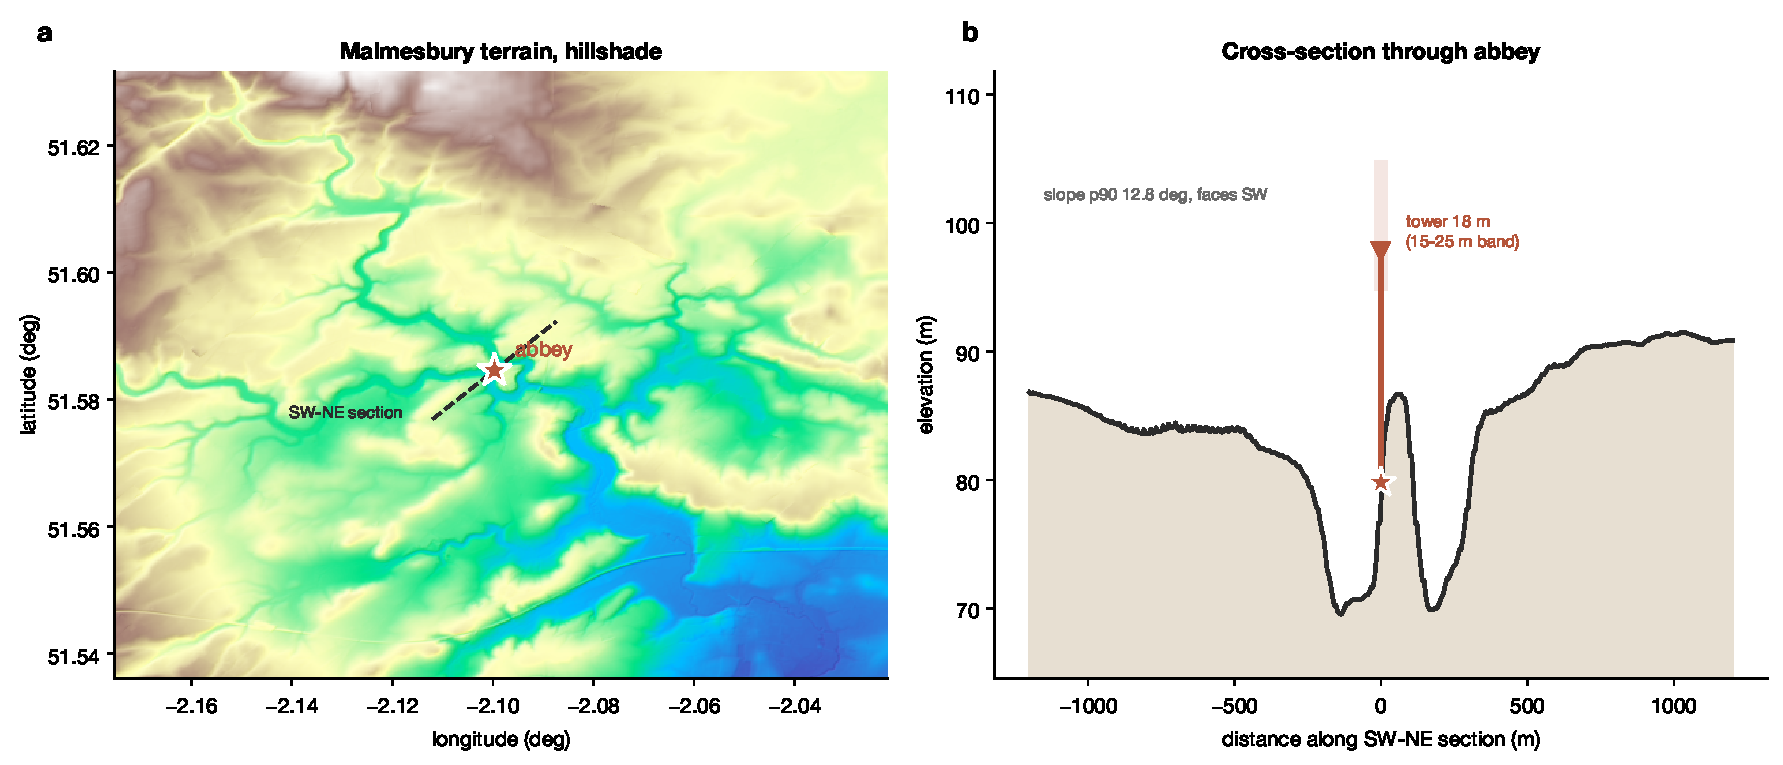
\includegraphics[width=\linewidth]{fig1_site}
  \caption{\textbf{Site and launch geometry at Malmesbury Abbey.}
  \textbf{(a)} Hillshaded terrain (AWS Terrain Tiles, about \SI{6}{\meter} posting)
  with the abbey on a promontory above the confluence of two Avon branches; the
  SW--NE line marks the section in (b).
  \textbf{(b)} Elevation along the section. The abbey stands \SI{10.2}{\meter} above
  the valley floor on a SW-facing slope (aspect \ang{230}; slope within
  \SI{400}{\meter}: mean \ang{5.2}, p90 \ang{12.8}).
  The \SI{6}{\meter} DEM under-resolves the launch edge, so the reported slope is a
  lower bound pending LIDAR.}
  \label{fig:site}
\end{figure}

\subsection{Favourable launch winds are common}

Over twenty years of ERA5 reanalysis, the wind blows from the SW sector at a
launchable \SIrange{5}{12}{\meter\per\second} in \SI{15.6}{\percent} of all hours
(\SI{95}{\percent} CI \numrange{14.3}{17.0}), about \num{1370} hours per year, with
a winter peak of \SI{21.1}{\percent} (\cref{fig:wind}).
The SW sector at any speed accounts for \SI{34.3}{\percent} of hours, so the
prevailing wind and the escarpment are well aligned.
A would-be flyer who waits for his conditions has them on the order of a thousand
hours a year, and the medieval wind regime appears no weaker than today's, so this
estimate is conservative for Eilmer's time.

\begin{figure}[htbp]
  \centering
  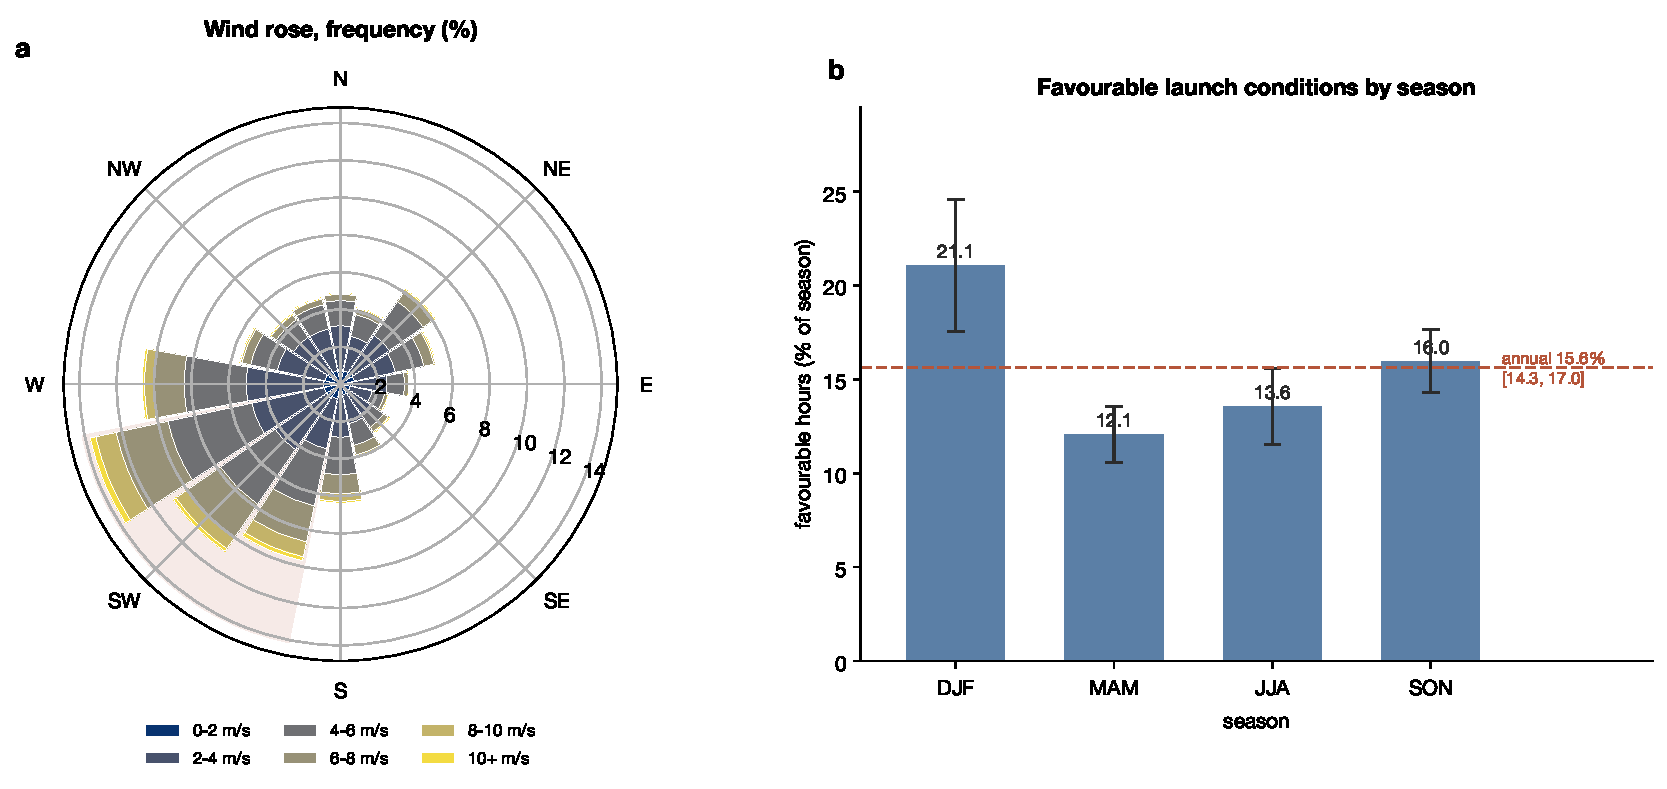
\includegraphics[width=\linewidth]{fig2_wind}
  \caption{\textbf{Favourable launch winds are common.}
  \textbf{(a)} Wind rose of ERA5 hourly \SI{10}{\meter} wind at the abbey,
  2004--2023 (\num{175320} hours).
  \textbf{(b)} Fraction of hours offering a favourable launch (SW sector
  \ang{191}--\ang{259} at \SIrange{5}{12}{\meter\per\second}), annually and by
  season, with \SI{95}{\percent} confidence intervals across the twenty years.
  Favourable conditions occur in \SI{15.6}{\percent} of hours (\SI{95}{\percent} CI
  \numrange{14.3}{17.0}), about \num{1370} hours per year, peaking in winter
  (\SI{21.1}{\percent}).}
  \label{fig:wind}
\end{figure}

\subsection{Ridge lift supplies the missing glide performance}

The linear orographic model (\cref{eq:ridge}) over the real terrain section gives a
peak upwash of about \SI{1.5}{\meter\per\second} just southwest of the abbey for an
\SI{8}{\meter\per\second} wind, with a soarable band about \SI{38}{\meter} deep
(\cref{fig:ridge}, supplementary).
That exceeds the optimistic sink of a crude glider
(\SIrange{0.75}{1.0}{\meter\per\second}), so the slope can in principle hold the
apparatus aloft, or at least flatten its descent, over the launch zone.
The mechanism is present and of the right order; with the smoothed DEM, both the
modelled slope and the lift it produces are lower bounds, which is why we keep the
full field in the supplement and carry only its magnitude into the glide analysis.

\subsection{A 200 m glide needs the wind}

In still air, covering \SI{200}{\meter} from an \SI{18}{\meter} tower demands a
glide ratio of \num{11.1}, which is sailplane class and far beyond a wood-and-cloth
wing (\cref{fig:glide}).
Adding the modelled ridge lift collapses the requirement: above
\SI{3.6}{\meter\per\second} of southwest wind the required glide ratio drops into
the crude cambered-wing band (\LD\ \numrange{3}{7}), reaching \num{4.8} at
\SI{8}{\meter\per\second}.
An \LD~5 wing launched into that wind clears \SI{200}{\meter} at about
\SI{7.5}{\meter\per\second}, inside the favourable band of \cref{fig:wind}.
The distance is achievable, but only with the wind and slope doing part of the work;
a calm-air leap from the tower would fall far short.

\begin{figure}[htbp]
  \centering
  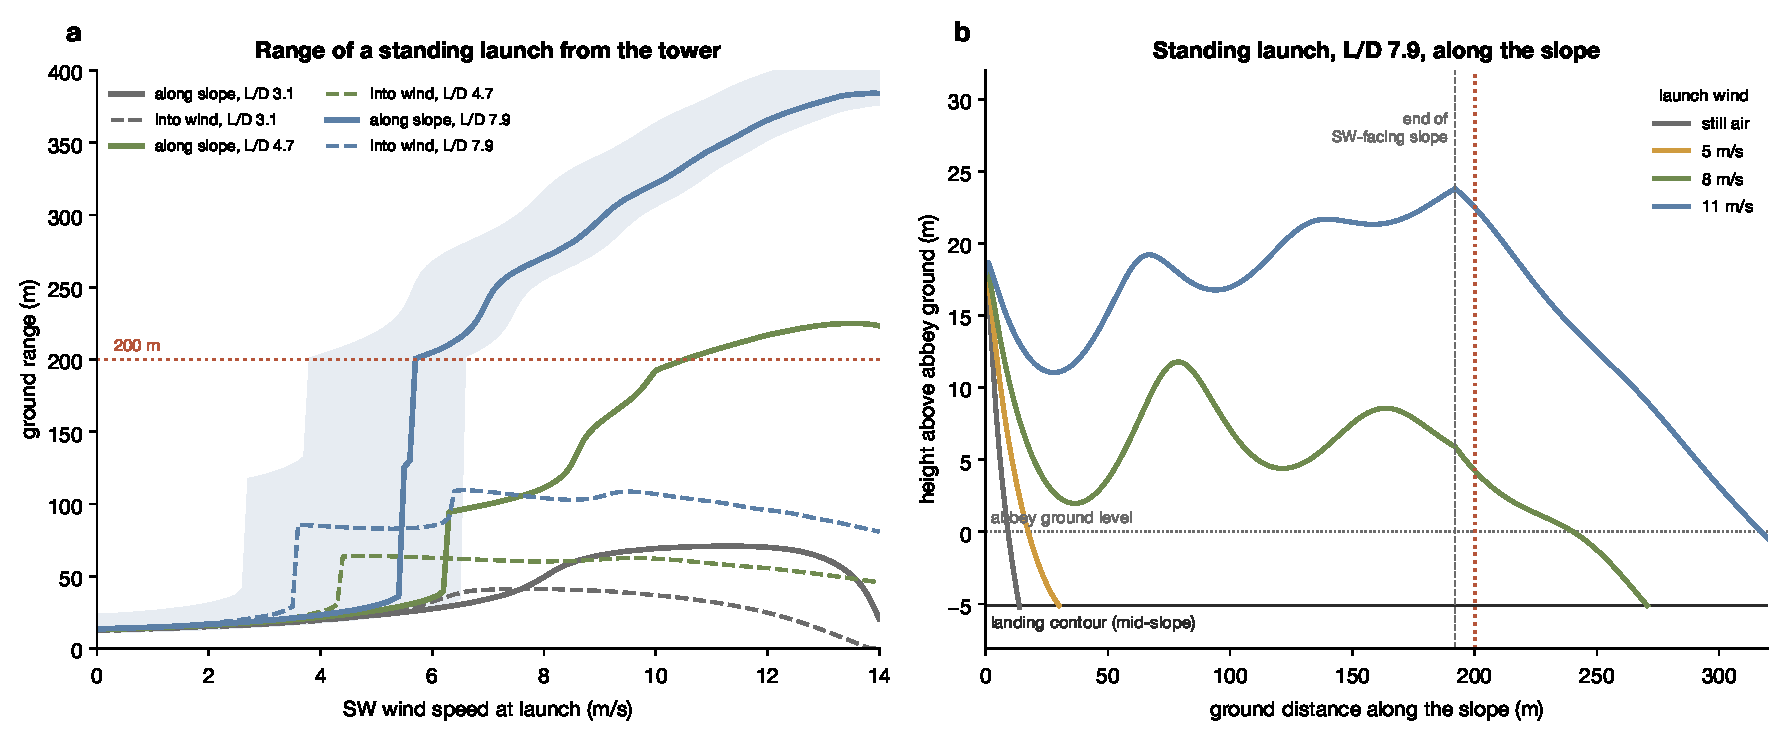
\includegraphics[width=\linewidth]{fig4_glide_envelope}
  \caption{\textbf{A \SI{200}{\meter} glide needs wind and slope.}
  \textbf{(a)} Range of an \LD~5 cambered wing launched from an \SI{18}{\meter}
  tower versus southwest wind speed; \SI{200}{\meter} is reached at about
  \SI{7.5}{\meter\per\second}.
  \textbf{(b)} Glide ratio required to cover \SI{200}{\meter} versus wind speed.
  Still air demands \LD~\num{11.1} (sailplane class, dotted line); with ridge lift
  the requirement falls into the crude cambered-wing band (\LD\ \numrange{3}{7})
  above \SI{3.6}{\meter\per\second}, reaching \LD~\num{4.8} at
  \SI{8}{\meter\per\second}.}
  \label{fig:glide}
\end{figure}

\subsection{The tailless craft cannot hold pitch}

A hanging pilot's CG (\numrange{0.35}{0.55}\,\(c\)) sits aft of a tailless wing's
neutral point (\(0.25\,c\)), so the configuration is statically unstable for every
posture the pilot can adopt (\cref{fig:stability}).
The instability is fast: after an \ang{8} gust the pitch attitude crosses the
\ang{60} loss-of-control threshold in \SI{0.74}{\second}, and the pitch error
doubles in \SIrange{0.1}{0.5}{\second} across the whole CG band, even with pitch
inertia varied by a factor of two, against a representative flight lasting
\SI{13.3}{\second}.
Fitting a tail moves the neutral point aft to \(0.53\,c\) and adds strong pitch
damping, which removes the divergence entirely.
The aerodynamics single out exactly the part Eilmer said he had left off.

\begin{figure}[htbp]
  \centering
  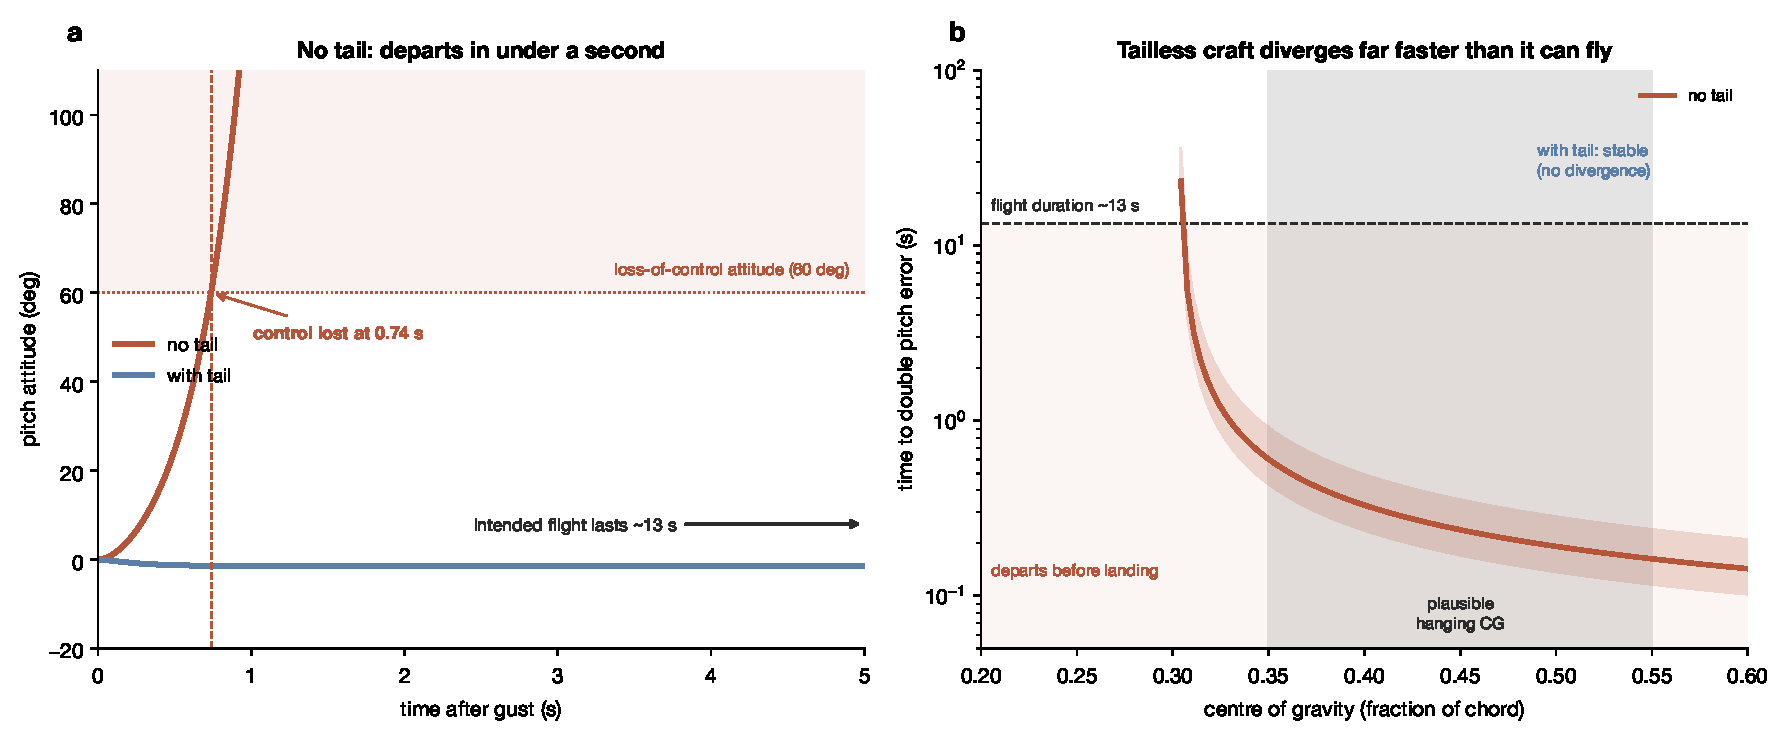
\includegraphics[width=\linewidth]{fig5_stability}
  \caption{\textbf{The tailless craft cannot hold pitch.}
  \textbf{(a)} Pitch-attitude response to an \ang{8} gust. Without a tail (red) the
  attitude crosses the \ang{60} loss-of-control line \SI{0.74}{\second} after the
  gust; with a tail (blue) the same gust damps out.
  \textbf{(b)} Time to double the pitch error across the plausible CG band:
  \SIrange{0.1}{0.5}{\second} everywhere for the tailless craft (pitch inertia
  varied \numrange{0.5}{2}\(\times\)), far shorter than the flight, and no
  divergence with a tail. A tail shifts the neutral point from \(0.25\,c\) to
  \(0.53\,c\), aft of a hanging pilot's CG (\numrange{0.35}{0.55}\,\(c\)).}
  \label{fig:stability}
\end{figure}

\subsection{The feasibility envelope}

Sampling the unknown apparatus and launch day \num{40000} times, \SI{27}{\percent}
of plausible worlds reach \SI{200}{\meter} (\SI{95}{\percent} CI \numrange{26}{27}),
with a median range of \SI{147}{\meter} (\cref{fig:montecarlo}a).
The typical draw falls short, but a furlong is far from rare, and Eilmer chose his
day and presumably his build, placing him in the upper tail.
Whether a reaching flight survives turns entirely on the tail, through a clean
timescale separation (\cref{fig:montecarlo}b): a tailless craft's pitch error
doubles in a median \SI{0.27}{\second} (p99 \SI{1.6}{\second}), with control lost
after about \SI{3}{\meter} of flight, while the glide must stay controlled for a
median \SI{20}{\second}, roughly \(75\times\) longer.
Every tailed configuration that reaches \SI{200}{\meter} is statically stable and
never diverges.
The model reproduces the reported sequence: he covered the distance, then lost
control.

\begin{figure}[htbp]
  \centering
  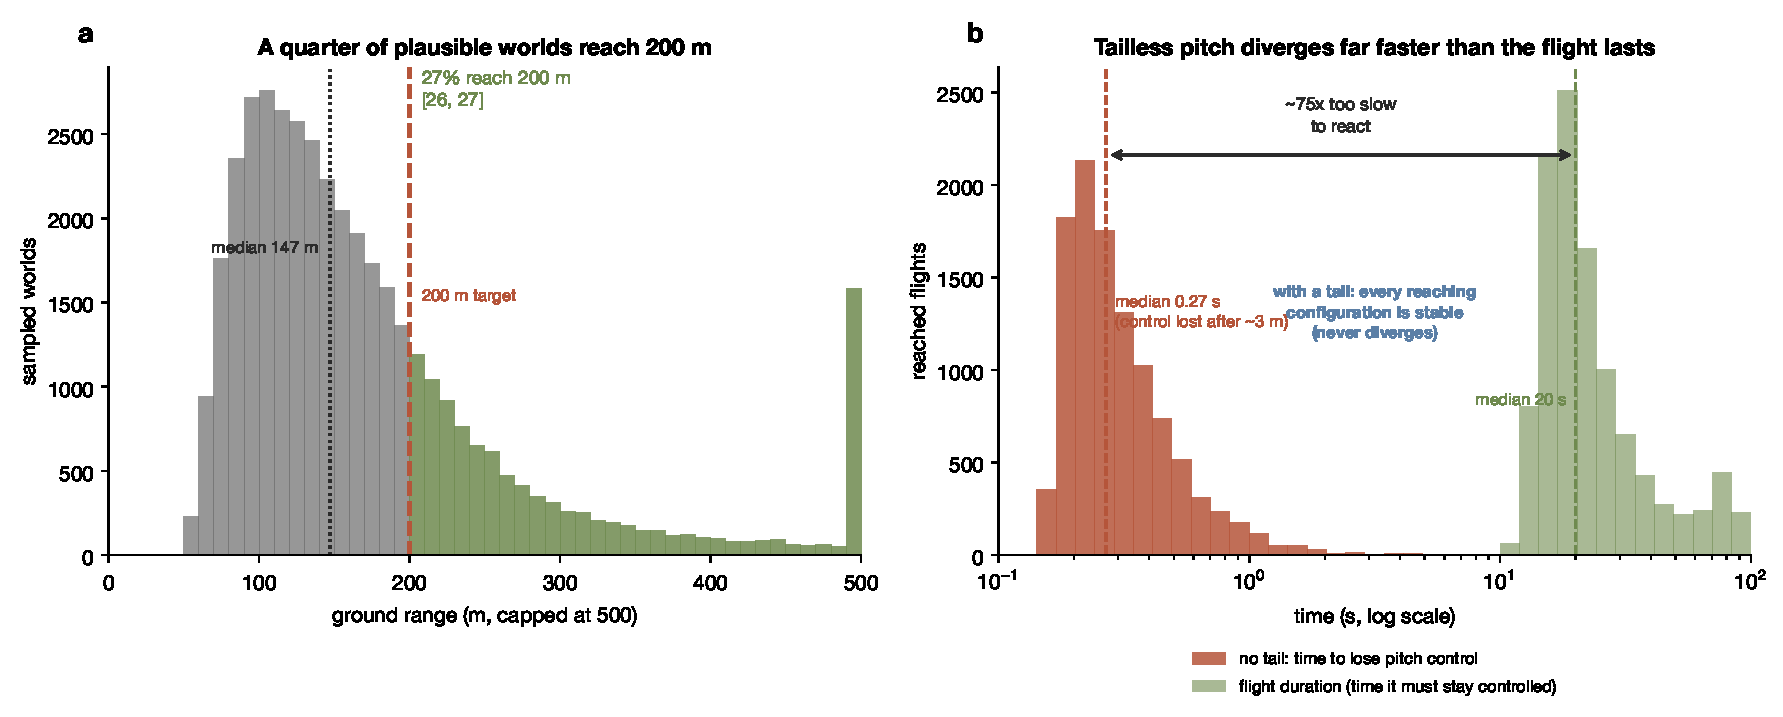
\includegraphics[width=\linewidth]{fig6_montecarlo}
  \caption{\textbf{Feasibility envelope over the unknown apparatus and day.}
  \num{40000} Monte Carlo samples drawing apparatus and launch parameters from
  plausible ranges, with launch wind drawn from the actual ERA5 SW-sector launchable
  speeds.
  \textbf{(a)} \SI{27}{\percent} of worlds reach \SI{200}{\meter} (\SI{95}{\percent}
  CI \numrange{26}{27}; median range \SI{147}{\meter}).
  \textbf{(b)} Among the reaching flights, tailless pitch error doubles in a median
  \SI{0.27}{\second} (p99 \SI{1.6}{\second}) against a flight that must stay
  controlled for a median \SI{20}{\second}, while tailed configurations never
  diverge.}
  \label{fig:montecarlo}
\end{figure}

\subsection{Broken legs fit an out-of-control arrival}

The reported injury is itself evidence (\cref{fig:biomech}).
A flared touchdown arrives at the sink rate (\SIrange{1}{3}{\meter\per\second}),
which is far below the tibia fracture-onset speed of about
\SI{9.7}{\meter\per\second} (range \numrange{7.5}{11.5}), so a controlled landing
could not break the legs.
An uncontrolled departure arrives near flying speed, with a vertical component of
\(V\sin\theta\), and breaks both tibiae with probability \num{0.66}, yet at about
\num{28}\,g over the legs it stays within the survivable feet-first regime rather
than the fatal one.
The injuries are thus positive evidence that Eilmer arrived out of control, the same
failure mode the missing tail predicts in \cref{fig:stability,fig:montecarlo}.

\begin{figure}[htbp]
  \centering
  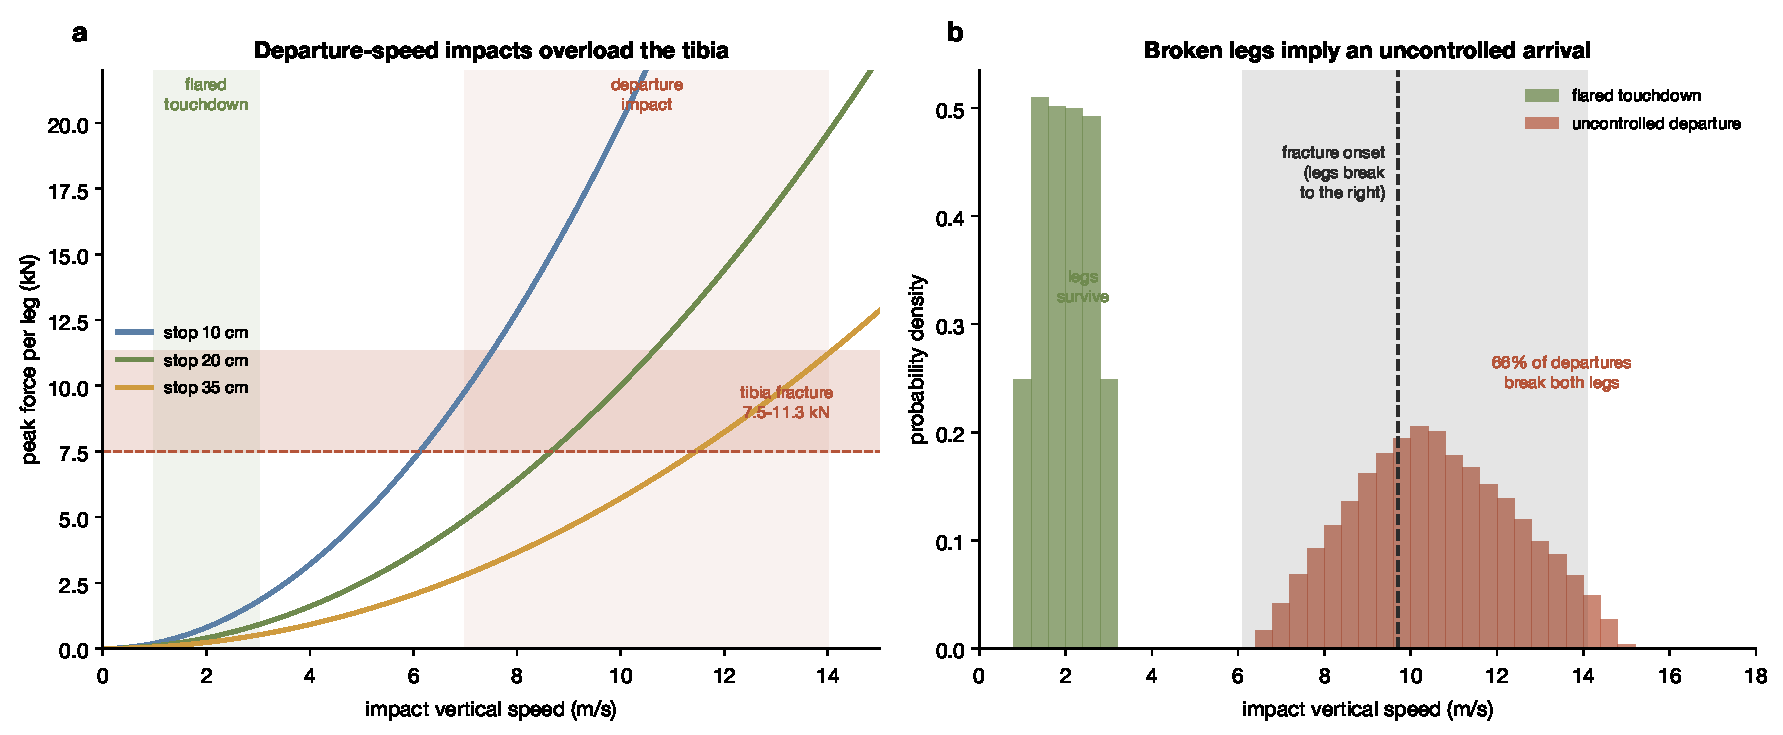
\includegraphics[width=\linewidth]{fig7_biomech}
  \caption{\textbf{Broken legs as evidence of an out-of-control arrival.}
  \textbf{(a)} Average feet-first impact force per leg versus vertical impact speed
  for ground-give distances \(d = \SIrange{10}{35}{\centi\meter}\), against the axial
  tibia fracture band (\SIrange{7.5}{11.3}{\kilo\newton} per leg). Fracture onset is
  about \SI{9.7}{\meter\per\second}.
  \textbf{(b)} Impact-speed distributions for a flared touchdown
  (\SIrange{1}{3}{\meter\per\second}) versus an uncontrolled departure
  (\(V\sin\theta\), \(V=\SIrange{11}{16}{\meter\per\second}\),
  \(\theta=\ang{35}\)--\ang{70}). A departure breaks both tibiae with probability
  \num{0.66} yet, at about \num{28}\,g, remains survivable.}
  \label{fig:biomech}
\end{figure}
\FloatBarrier
